\subsection{User Management}
This module is responsible for reading data from the client user database. It will do this by making use of ldap.js .
\subsubsection{Scope}
\paragraph{Test}
\subsubsection{Use cases}
\begin{itemize}
\item Autorize
\item validateUserName
\item retrieveEmail
\end{itemize}
\subsubsection{Domain model}
\subsection{Project}
\subsubsection{Scope}
\subsubsection{Use cases}
\subsubsection{Domain model}
\subsection{Estimation}
\subsubsection{Scope}
\subsubsection{Use cases}
\subsubsection{Domain model}
\subsection{Report}
The Report module will do statistical analysis on the data as well as draw graphs of the estimation data. This module will be responsible for any analysis of the data. It's functionality will be expanded as development continues.
\subsubsection{Scope}
The scope of this module will be accessible to any user at this point in the development, the only authorization that will take place is the initial log in of the user.
	\begin{figure}[H]
	    	\centering
	    	\fbox{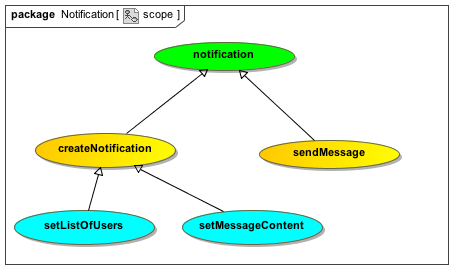
\includegraphics[width=0.8\textwidth]{Notification_Scope}}
	    	\caption{Report Scope}
	    	\label{fig:Report_Scope.png}
   	\end{figure}
\subsubsection{Use cases}
	\paragraph{Statistical Analysis: critical}
	User accessing this function will receive statistical analysis of the data for the chosen project.

	\paragraph{Generate Graphs: critical}
	User accessing this function will receive a series of graphs of the data for the chosen project. 
\subsubsection{Domain model}
\subsection{Notification}
\subsubsection{Scope}
\subsubsection{Use cases}
\subsubsection{Domain model}
